\documentclass[tikz,border=8pt]{standalone}
% Shared look for every TikZ diagram. Load with \input{../../tools/tikz-style.tex}
\usepackage[T1]{fontenc}
\usepackage{lmodern}
\renewcommand{\sfdefault}{lmr}  % diagrams use the same serif as the text
\usetikzlibrary{arrows.meta, positioning, shapes.geometric, calc, fit, backgrounds}
\definecolor{cblue}{HTML}{4C78A8}
\definecolor{corange}{HTML}{F58518}
\definecolor{cgreen}{HTML}{54A24B}
\definecolor{cred}{HTML}{E45756}
\definecolor{cpurple}{HTML}{B279A2}
\definecolor{cgrey}{HTML}{6B6B6B}
\tikzset{
  every picture/.style={font=\sffamily, line width=1.2pt},
  box/.style={draw=#1, fill=#1!12, rounded corners=4pt, align=center, inner sep=7pt, minimum height=1.1cm},
  box/.default=cgrey,
  arrow/.style={-{Stealth[length=3mm]}, draw=cgrey, line width=1.4pt},
  title/.style={font=\sffamily\bfseries\Large},
  note/.style={font=\sffamily\small, text=cgrey, align=center},
}
\AtBeginDocument{\hyphenpenalty=10000 \exhyphenpenalty=10000}

\begin{document}
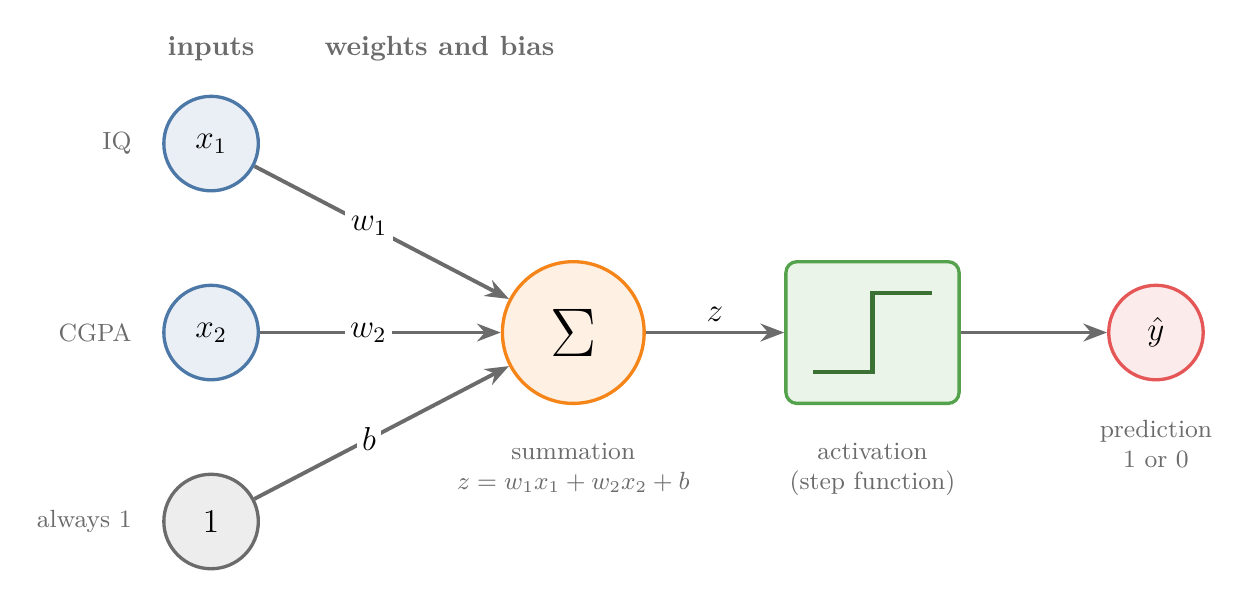
\begin{tikzpicture}
  \tikzset{inp/.style={circle, draw=cblue, fill=cblue!12, minimum size=1.2cm, font=\sffamily\large},
           wl/.style={font=\sffamily\large, fill=white, inner sep=2pt}}
  \node[inp] (x1) at (0,2.4) {$x_1$};
  \node[inp] (x2) at (0,0) {$x_2$};
  \node[inp, draw=cgrey, fill=cgrey!12] (one) at (0,-2.4) {$1$};
  \node[note, left=0.25cm of x1] {IQ};
  \node[note, left=0.25cm of x2] {CGPA};
  \node[note, left=0.25cm of one] {always 1};
  \node[circle, draw=corange, fill=corange!12, minimum size=1.8cm, font=\sffamily\Huge] (sum) at (4.6,0) {$\Sigma$};
  \node[box=cgreen, minimum width=2.2cm, minimum height=1.8cm] (act) at (8.4,0) {};
  \draw[cgreen!70!black, line width=1.6pt] ([xshift=-0.75cm,yshift=-0.5cm]act.center) -- ([yshift=-0.5cm]act.center) -- ([yshift=0.5cm]act.center) -- ([xshift=0.75cm,yshift=0.5cm]act.center);
  \node[inp, draw=cred, fill=cred!12] (out) at (12,0) {$\hat{y}$};
  \draw[arrow] (x1) -- node[wl, pos=0.45] {$w_1$} (sum);
  \draw[arrow] (x2) -- node[wl, pos=0.45] {$w_2$} (sum);
  \draw[arrow] (one) -- node[wl, pos=0.45] {$b$} (sum);
  \draw[arrow] (sum) -- node[above, font=\sffamily\large] {$z$} (act);
  \draw[arrow] (act) -- (out);
  \node[note, below=0.35cm of sum] {summation\\$z = w_1x_1 + w_2x_2 + b$};
  \node[note, below=0.35cm of act] {activation\\(step function)};
  \node[note, below=0.35cm of out] {prediction\\1 or 0};
  \node[note, font=\sffamily\bfseries] at (0,3.6) {inputs};
  \node[note, font=\sffamily\bfseries] at (2.9,3.6) {weights and bias};
\end{tikzpicture}
\end{document}
